\subsection{SimpleCNN}\label{resultsSimpleCNN}

After establishing the basic architecture of our SimpleCNN (as described in Section~\ref{simplecnn}), our next goal was to effectively classify the first digits of the dataset. This required the selection of initial hyperparameters to begin the training and evaluation process. Without prior benchmarks, we initially decided on a batch size of 8, set the number of epochs to 5 and a learning rate of 0.1. However, this initial configuration led to less satisfactory results, prompting us to revise our hyperparameters to improve performance.

The training process was completed relatively quickly, which prompted us to implement a function to test the hyperparameters. This required us to set default values for each training and evaluation session, with certain values being adjusted at each iteration. For example, we set the batch size to 32, the learning rate to 0.001 and the epochs to 15. In subsequent runs, we changed one hyperparameter at a time, while keeping the others constant. This means that we ran training sessions with learning rates of 0.001, 0.01 and 0.1, respectively, while keeping the default values for batch size and epochs. Similarly, we experimented with different batch sizes and varied the number of epochs. This systematic approach allowed us to evaluate the effects of each hyperparameter. The following code snippedt provides a brief summary of the hyperparameters that were explored during this process:

\begin{minted}[mathescape, linenos, fontsize=\small]
{python}
    ...
    # Hyperparameters
    num_classes = 10
    default_lr = 0.001
    default_bs = 32
    default_epoch = 15
    learning_rates = [default_lr, 0.01, 0.1]
    batch_sizes = [16, default_bs, 64]
    num_epochs = [5, 10, default_epoch, 20]
    ...
\end{minted}

Upon reviewing the experiment results in Table~\ref{table:lr_bs_ep}, we identified the optimal hyperparameters for our SimpleCNN model, surprisingly finding that default values already yielded the best outcomes.


\begin{table}[ht]
  \caption{Impact of Learning Rate, Batch Size, and Epochs on Accuracy}\label{table:lr_bs_ep}
  \centering
  \begin{tabular}{lll}
  \toprule
  \addlinespace
  \multicolumn{3}{c}{Learning Rate} \\
  \midrule
  Learning Rate & Average Train Accuracy (\%) & Average Validation Accuracy (\%) \\
  \midrule
  0.001 & 99.6 & 98.9 \\
  0.01  & 97.7 & 97.2 \\
  0.1   & 10.3 & 10.0 \\
  \midrule
  \addlinespace
  \addlinespace
  \multicolumn{3}{c}{Batch Size} \\
  \midrule
  Batch Size & Average Train Accuracy (\%) & Average Validation Accuracy (\%) \\
  \midrule
  16 & 99.7 & 98.9 \\
  32 & 99.5 & 98.9 \\
  64 & 99.4 & 98.9 \\
  \midrule
  \addlinespace
  \addlinespace
  \multicolumn{3}{c}{Epochs} \\
  \midrule
  Epochs & Average Train Accuracy (\%) & Average Validation Accuracy (\%) \\
  \midrule
  5  & 99.4 & 98.8 \\
  10 & 99.6 & 99.0 \\
  15 & 99.6 & 99.0 \\
  20 & 99.7 & 99.0 \\
  \bottomrule
  \end{tabular}
  \end{table}
  

The above results were all optained using the initial SimpleCNN architecture. The adpated, newer version of the SimpleCNN was also then trained using the best hyperparameters determined. In order to evaluate the effectiveness of the changes, we compared the performance of both architectures. The results can be seen in Figure~\ref{fig:SimpleCNN_old_new}.

%\begin{table}[ht]
%  \caption{Comparison of Initial and Adapted SimpleCNN on MNIST}\label{table:comparison-simplecnn}
%  \centering
%  \begin{tabular}{cccccc}
%  \toprule
%  Epoch & \multicolumn{2}{c}{Initial SimpleCNN} & & \multicolumn{2}{c}{Adapted SimpleCNN} \\
%  \cmidrule{2-3} \cmidrule{5-6}
%   & Train Loss & Validation Accuracy (\%) & & Train Loss & Validation Accuracy (\%) \\
%  \midrule
%  1  & 0.1043 & 97.49 & & 0.0203 & 98.82 \\
%  2  & 0.0239 & 98.16 & & 0.0045 & 99.01 \\
%  3  & 0.0025 & 98.71 & & 0.1208 & 99.13 \\
%  4  & 0.3143 & 98.68 & & 0.0504 & 99.22 \\
%  5  & 0.1803 & 98.76 & & 0.0316 & 99.29 \\
%  6  & 0.0221 & 98.73 & & 0.1246 & 99.24 \\
%  7  & 0.0000 & 98.83 & & 0.0014 & 99.38 \\
%  8  & 0.0001 & 98.94 & & 0.0021 & 99.19 \\
%  9  & 0.0000 & 98.85 & & 0.0087 & 99.42 \\
%  10 & 0.0176 & 99.03 & & 0.0001 & 99.42 \\
%  11 & 0.0011 & 98.90 & & 0.0076 & 99.46 \\
%  12 & 0.0014 & 98.75 & & 0.0005 & 99.41 \\
%  13 & 0.0000 & 98.88 & & 0.0119 & 99.44 \\
%  14 & 0.0000 & 99.04 & & 0.0296 & 99.38 \\
%  15 & 0.0261 & 99.09 & & 0.0075 & 99.49 \\
%  \bottomrule
%  \end{tabular}
%  \end{table}

  \begin{figure} [ht]
    \centering
    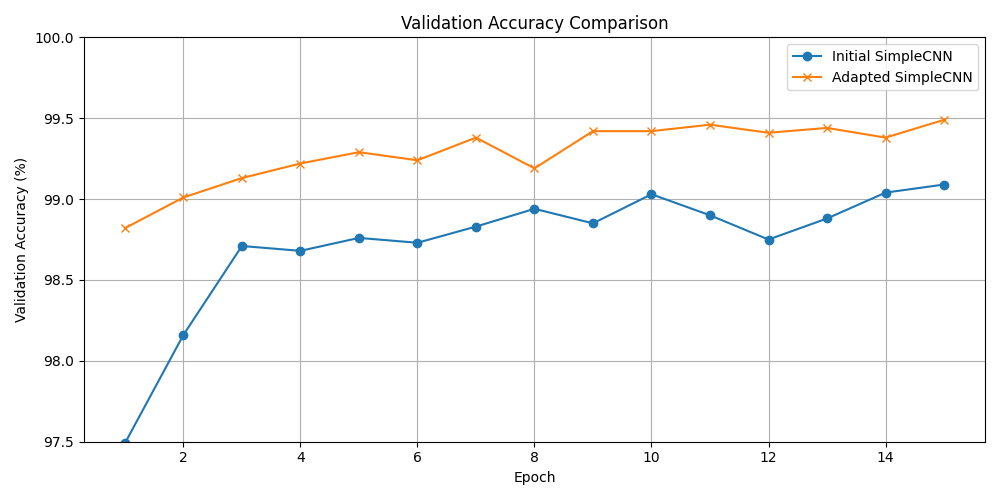
\includegraphics[width=.9\textwidth]{figures/simpleCNN_old_vs_new.png}
    \caption{Comparison of validation accuracy across epochs between the initial and the adapted SimpleCNN model, highlighting the overall improved performance of the adapted model.}\label{fig:SimpleCNN_old_new}
\end{figure}

For the second challenge, which focused on the PathMNIST dataset, our approach exclusively employed the adapted version of our SimpleCNN architecture due to its improved performance. To combat overfitting, we introduced an early stopping mechanism. The core of this experiment was to assess the impact of incorporating batch normalization and dropout techniques. We conducted three separate trials: one with both batch normalization and dropout, one with only dropout, and another with only batch normalization. The outcomes of these trials can be seen in Figures .